\subsubsection{Ecological Genomics}
\index{Gl�ckner, Frank Oliver}

\paragraph{Research Team}
%
Frank Oliver Gl�ckner (Professor), Marga Bauer (Postdoc), Thierry Lombardot (Postdoc), Francesca Simonata (Postdoc), Hanno Teeling (Postdoc),  Marcel Huntemann (PhD Student), Renzo Kottmann (PhD Student), Christian Quast (PhD Student), Michael Richter (PhD Student), Patricia Wecker (PhD Student), J�rg Peplies (Guest), Andreas Ellrott (Technical Assistant), Carsten Witt (Technical Assistant)\\

The advent of high throughput sequencing technologies in the last years enables to unravel the diversity and function of marine microorganisms on a whole genome level. It's the objective of Genome Bioinformatics to take advantage of this development and learn more about the mechanisms coded in the genome enabling the organisms to adapt to changing environmental conditions. To reveal the relevant genes and their functions an integrative approach is followed to correlate sequence data with information about gene expression, habitat-specific parameters and microbial diversity. This in turn should uncover specific niche adaptations and give hints how the organisms influence the global cycling of matters. The knowledge obtained will lead to a better understanding of the complexity, interactions and stability of marine habitats. The long-term perspective is to predict the impact of the ongoing global changes on the marine ecosystem.

\paragraph{Highlights}


\textit{Genomics and Metagenomics}
One of the highlights in 2006 was the contribution to the paper by Woyke et al. which came out in Nature recently. In this metagenomic paper random shot gun sequencing was used to address the metabolic potential of the symbiotic community of the marine worm \textit{Olavius algarvensis}. Besides enhanced functional annotation, we were able to further address the binning problem, which is central to any metagenomic project. Binning means the bioinformatic assignment of the sequence fragments back to the organisms in the sample. The problems are: 1. the sequence fragments that carry the metabolic genes of interest often lack suitable markers for their phylogenetic classification, and 2. fragments from the same organism can not be reliably identified as such, unless they overlap. The tool TETRA (www.megx.net/tetra) has been developed to address this task based on intrinsic sequence signatures and successfully applied in several projects. Since it is limited to fragment sizes above 20-30 kb we have further developed the system to enhance sensitivity. The new MetaClust system is now able to deal with fragment sizes down to 5 kb. A prototype of the new system was evaluated within the \textit{O. algarvensis} project and the four expected symbiotic genomes could be clearly differentiated (see Figure \ref{fig:gloeckner-fig1}).
Additionally, we could finish four genome projects that provided new insights into the life-style of three marine bacteria and one marine phage. All projects have been performed in close collaboration with national and international partners from the Network of Excellence Marine Genomics Europe and the Joint Genome Institute in the US.

Within the framework of our EU-project MetaFunctions (www.metafunctions.org) we were able to significantly enhance the integrative database and our visualization tools provided by the `Genomes Mapserver' (www.megx.net/mm). The idea behind MetaFunctions is to integrate sequence data with habitat parameters using the geographic information system (GIS). The ultimate aim is to use novel data-mining systems that help determining functions of those genes for which the activity is not yet known. Hundred thousand of scientific publications and the public sequence repositories are now screened by our partners for relevant information. A variety of natural language processing algorithms are being tested to collate this data and convert it into our structured, database format. Analytical tools like MetaLook are under development to enable the project team and later scientists around the world to clearly visualize the results of diverse analyses.
\begin{figure}[ht]
  \begin{center}
   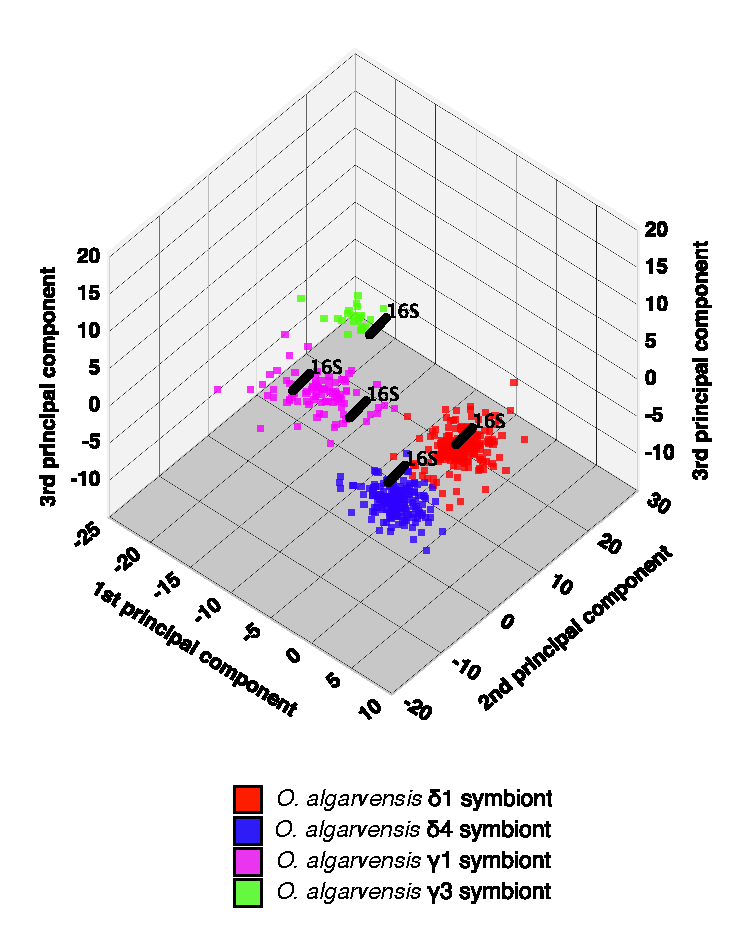
\includegraphics[width=\hsize]{Gloeckner/Gloeckner-fig1.pdf}
    \mycaption{Clustering of the \textit{O. algarvensis} symbiont scaffolds. Visualization
of the first three components of a principal component analysis, in
which GC-content, net-read-depth z-scores for all possible 64
trinucleotides and 256 tetranucleotides were incorporated with equal
weight (z-scores calculated with TETRA, and normalized by length).
The colours represent the four clusters of scaffolds (calculated
with MetaClust). }\label{fig:gloeckner-fig1}
   \end{center}
\end{figure}

\textit{Microarray analysis}
Systematic studies have been conducted to address the issue of nonspecific target binding. This was possible in collaboration with Dirk Sch�ler from the MPI-Bremen since he was able to provide the isogenic deletion mutant MSR-1B of \textit{Magnetospirillum gryphiswaldense}. This model system was used to systematically investigate the amount of false positive hybridization events. Finally, a three colour hybridization assay was developed to compare MSR-1B culture and two MSR-1 wild type cultures grown under different conditions. The results show that common microarray platforms still suffer from a significant amount of unspecific signals even under optimal hybridization conditions.



\paragraph{Organization}
%
\begin{enumerate}
\item EU-workshop Bioinformatics I - Introduction to Sequence and Genome Analysis in collaboration with the Ribocon GmbH (January 23-27)
\item Extended international phylogeny (ARB) workshop in collaboration with the Ribocon GmbH (May 30 - June 02)
\item International Exploratory Workshop: ``Marine Genomics meets Marine Diversity'' (June 07-09)
\item International phylogeny (ARB) workshop in Z�rich in collaboration with the Ribocon GmbH (September 19-22)
\item International phylogeny (ARB) workshop in collaboration with the Ribocon GmbH (November 28 - December 02)
\end{enumerate}

\myparagraph{Collaborations}
%
Bremen Area Collaborations:
\begin{enumerate}
\item {\sl International University Bremen} \\ Prof. M.-Th. H�tt \\ Genome signatures
 \\ Prof. G. Muskhelishvili \\ Transcriptomics
\\ Prof. M. Ullrich \\Expression profiling
\\ Prof. M. Zacharias, Prof. U. Schwaneberg\\ Sulfatases
\item {\sl Universit�t Bremen} \\ Prof. O. Herzog \\ Bioinformatics
\item {\sl TTZ Bremerhaven} \\ Dr. U. Bohnebeck \\ MarMic, Metafunctions
\item {\sl University Hamburg} \\ Prof. S. Kurtz \\ Genomics
\item {\sl Alfred-Wegener-Institut Bremerhaven} \\ Wilshire \\ LTER
\end{enumerate}
National \& International Collaborations:
\begin{enumerate}
\item {\sl Technische Universit�t M�nchen} \\ Dr. W. Ludwig\\ Bioinformatics, ARB, ARB-Genome
\item {\sl Universit�t Bielefeld} \\ Prof. A. P�hler, Dr. A. Becker\\ Bioinformatics, GenDB, microarrays
\item {\sl University W�rzburg} \\ Dr. U. Hentschel\\ Phylogeny
\item {\sl Max-Planck-Institut f�r molekulare Genetik, Berlin} \\ Dr. R. Reinhard\\ Genome sequencing
\item {\sl Rechenzentrum der MPG Garching} \\ Dr. H. Lederer\\ Bioinformatic pipeline
\item {\sl Bundesanstalt f�r Gew�sserkunde} \\ Dr. W. Manz\\ Microarrays
\item {\sl University of the Balearic Islands} \\ Prof. R. Rossello-Mora\\ Molecular taxonomy and ecology, Salinibacter
\item {\sl University of Alicante} \\ Prof. P. Anton\\ Salinibacter
\item {\sl Station Biologique Roscoff} \\ Dr. G. Michel\\ Zobellia
\item {\sl CBS Danmark} \\ Prof. D. Ussery\\ genome comparison
\item {\sl Woods Hole Marine Biological Laboratory} \\ Prof. M. Sogin, D. L-A. Zettler\\ ICoMM
\item {\sl UNEP/GRID-Europe} \\ Dr. J. Jaquet \\ Metafunctions
\item {\sl Poznan University of Technology} \\ Prof. J. Blazewicz \\ Metafunctions
\end{enumerate}

\paragraph{Grants at the Max Planck Institute for Marine Microbiology}
\begin{enumerate}
\item EU-NoE Marine Genomics Europe (GUCE-CT-2004-505403)
\item EU-project MetaFunctions (511784-2)
\end{enumerate}

\goodbreak

\nocite{Gloeckner1,Gloeckner2,Gloeckner3,Gloeckner4,Gloeckner5,Gloeckner6,Gloeckner7,Gloeckner8,Gloeckner9,Gloeckner10,Gloeckner11,Gloeckner12}
